\documentclass{article}
\usepackage{amsmath}
\usepackage{amsfonts}
\usepackage{amssymb}
\usepackage{enumitem}
\usepackage{tikz}
\usepackage{mathtools}

\usetikzlibrary{arrows}

\title{CSC 226 - Assignment 4 - Theory}
\date{April 2017}
\author{Daniel Frankcom}

\begin{document}
	\pagenumbering{gobble}
	\maketitle
	\setlength{\parindent}{0pt}
	\newcommand{\forceindent}{\leavevmode{\parindent=72pt\indent}}
	\newpage
	\pagenumbering{arabic}
	
	\begin{enumerate}
		\item 
		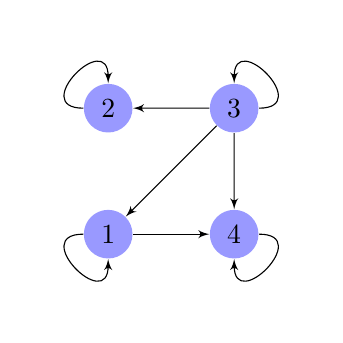
\begin{tikzpicture}
		[scale=.8,auto=left,every node/.style={circle,fill=blue!40}, edge/.style={->,> = latex'}]
		\node (n1) at (0,0)  {1};
		\node (n2) at (0,2)  {2};
		\node (n3) at (2,2)  {3};
		\node (n4) at (2,0)  {4};
		
		\foreach \from/\to in {n1/n4,n3/n4,n3/n1,n3/n2}
		\draw[edge] (\from) to (\to);
		
		\draw[edge] (n1) to [out=180,in=270,looseness=4] (n1);
		\draw[edge] (n2) to [out=180,in=90,looseness=4] (n2);
		\draw[edge] (n3) to [out=360,in=90,looseness=4] (n3);
		\draw[edge] (n4) to [out=360,in=270,looseness=4] (n4);
		\end{tikzpicture}
	\end{enumerate}
\end{document}